\apendice{Especificación de requisitos} \label{Ap:requisitos}

\section{Introducción}

En este apéndice se exponen los requisitos del software creado y la funcionalidad de este. Para ello, se da un descripción completa de las funciones que debe realizar el programa y de cómo un usuario podría utilizarlo. Se definen los pasos y opciones para utilizar correctamente el hardware del sistema empotrado y que cumpla así con su función. Por otro lado, se definen también los requisitos no funcionales. Para la exposición de estos requisitos se seguirán algunos estándares como el IEEE 830\-1998 \cite{IEEE8301998} o el IEEE 29148\-2011 \cite{IEEE291482011}.

\subsection{Audiencia destinataria}
Este documento tiene como destinatario, cualquier persona que quiera iniciarse en el ámbito de los sistemas embebidos. Tanto alumnos, como profesores u otros usuarios interesados, podrán encontrar información sobre comunicaciones con periféricos y entre SE, y para qué y cómo pueden utilizarse. 

Para la exposición de las siguientes secciones se utilizarán, por motivo de simplicidad, algunas abreviaciones:
\begin{description}
\item[Sistema empotrado o embebido.] SE
\item[Software del sistema empotrado.] SW del SE
\item[Requisito de interfaces externas.] RE
\item[Requisito funcional.] RF
\item[Requisito no funcional.] RNF
\item[Casos de Uso.] CU
\end{description}

\subsection{Objetivos generales}
En esta sección vamos a ver los objetivos para el funcionamiento del SE:
\begin{itemize}
\item Configurar un SE para que pueda conectarse en red mediante cable y comunicarse utilizando TCP/IP 
\item Gestionar el hardware de la planta piloto mediante envío de comandos software entre placas
\end{itemize}
A partir de estos dos objetivos principales vamos a continuar viendo en los demás apartados los requisitos que tiene la planta piloto.

\subsection{Tipos de usuario}
Para la utilización del sistema empotrado no se necesita ningún tipo de conocimiento técnico por lo que cualquier persona interesada puede usarlo sin problemas. La mayor dificultad radica en conectar los componentes correctamente, conocer los casos de uso del SE y los pasos para utilizar la placa `maestro'. 
Teniendo en cuenta que junto con el software se proporcionan varios documentos:
\begin{itemize}
\item Manual del usuario.
\item Manual del programador.
\item Casos de uso de la planta piloto.
\end{itemize} 
Cualquier usuario podría utilizarlo atendiendo a esos documentos.

\section{Catálogo de requisitos}
\subsection{Requisitos externos}
\begin{itemize}
  	
	\item \textbf{RE-1 Acceso a la red.} El SE tiene que ser capaz de usar Ethernet para conectarse en red. RE de alta prioridad.
	\item \textbf{RE-2 Transmisiones en red.} El SE tiene que ser capaz de usar el protocolo TCP/IP para comunicarse con otros sistemas embebidos. RE de alta prioridad.
	\item \textbf{RE-3 Uso de Botones.} Los seis botones disponibles en la placa más el shield deben poderse utilizar correctamente.  RE de media prioridad.
	\item \textbf{RE-4 Uso de dispositivos ADC.} Tanto el sensor de temperatura como los potenciómetros deben realizar adecuadamente sus lecturas. RE de alta prioridad.
	\item \textbf{RE-5 Uso de pantalla LCD} La pantalla debe mostrar los mensajes requeridos correctamente. RE de media prioridad
	
\end{itemize}

\subsection{Requisitos Funcionales}
\begin{itemize}
  	\item \textbf{RF-1 Recepción de comandos} El SE tiene que recibir comandos transmitidos mediante paquetes TCP con destino a su correspondiente dirección IP y puerto TCP abierto. RF de alta prioridad.
  	\item \textbf{RF-2 Identificación de comandos} El SE tiene que ser capaz de identificar los comandos recibidos para poder ejecutar las acciones correctas. RF de alta prioridad
  	\item \textbf{RF-3 Movimiento de los motores} Los motores deben realizar correctamente su giro dependiendo del comando recibido. RF de alta prioridad.
  	\item \textbf{RF-4 Obtención de la velocidad de los motores} La obtención de los valores de velocidad de los motores debe ser recibida sin demora y correctamente. RF de media prioridad.
  	\item \textbf{RF-5 Obtención de la temperatura} La obtención de los valores de temperatura debe ser recibida sin demora y correctamente. RF de media prioridad.
  	\item \textbf{RF-6 Envío de comandos} Los comandos se deben enviar por red y no deben perderse en el proceso de comunicación. RF de alta prioridad.
  	\item \textbf{RF-7 Parada de ambos motores} La parada de ambos motores al pulsar el `botón de emergencia' debe ser rápida y completa. RF de alta prioridad.
  	\item \textbf{RF-8 Comunicación I2C} La comunicación con la pantalla LCD debe ser mediante I2C. RF de alta prioridad.
	\item \textbf{RF-9 comunicación UART} La comunicación con los motores mediante UART debe ser rápida y confiable. RF de alta prioridad.
\end{itemize}

\subsection{Requisitos No Funcionales}
\begin{itemize}
  	\item \textbf{RNF-1 Hardware del SE} El SE tiene que ser desarrollado con una placa de desarrollo FRDM-K64F. RNF de alta prioridad.
  	\item \textbf{RNF-2 Rendimiento del SE} El SE tiene que ser capaz de realizar las acciones indicadas por el usuario sin demora. RNF de media prioridad.
  	\item \textbf{RNF-3 Seguridad del SE} El SE tiene que asegurar que sus componentes no presentan riesgos eléctricos al usuario. RNF de alta prioridad. 
  	\item \textbf{RNF-4 Calidad del SW} El SW tiene que garantizar cierto nivel de calidad, tales como incluir comentarios que faciliten su comprensión para un mantenimiento o portabilidad posteriores. RNF de media prioridad.
  	\item \textbf{RNF-5 Usabilidad del SE} La utilización del sistema debe ser sencilla para el usuario. RNF de alta prioridad.
  	\item \textbf{RNF-6 Conectividad física de los componentes} Los elementos que componen el sistema deben estar conectados de manera adecuada. RNF de alta prioridad.
\end{itemize}



\section{Especificación de requisitos}

\subsection{Diagrama de Casos de Uso}

En la figura \ref{casosDeUso} se muestran los casos de uso que un usuario puede llevar a cabo con la planta piloto.

%\imagen{casosUso}{Diagrama de casos de uso.} \label{casosDeUso}
\begin{figure}[H]%
    \begin{center}%
    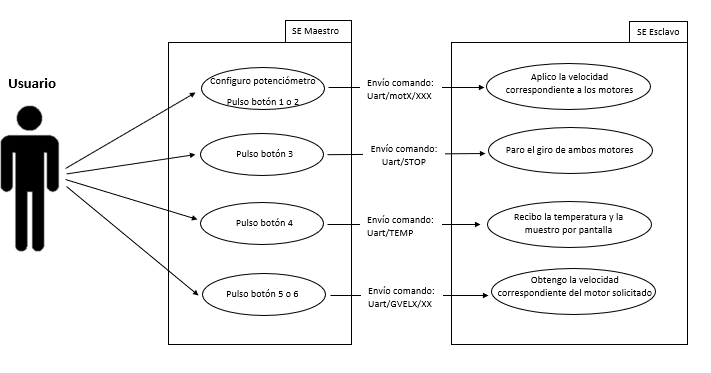
\includegraphics[angle=90,width=0.6\textwidth]{casosUso}%
    \caption{Diagrama de casos de uso.}%
    \label{casosDeUso}%
    \end{center}%
  \end{figure}%

\subsection{Casos de Uso}
Las siguientes tablas muestran los requisitos de los casos de uso:

\tablaSmallSinColores{CU-1 Set Speed A.}{l l}{cu-1}
{\multicolumn{1}{l}
{CU-1}                          & Set Speed A \\}
{ 
  \textbf{Versión}              & 1.0     \\
  \textbf{Fecha}                & 2022-06 \\
  \textbf{Requisitos asociados} & RF-3   \\
  \textbf{Descripción}          & Fijar la velocidad del Motor A\\ 
  \textbf{Precondición}         & \parbox{.5\textwidth}{\begin{itemize}
  	\item Se debe tener conexión en red entre las placas.
    \item Todos los elementos del sistema deben estar conectados
    \end{itemize}}\\
  \textbf{Acciones}             & \parbox{.5\textwidth}{\begin{enumerate}
    \item El usuario ajusta el potenciómetro 1 según sus necesidades.                         
    \item El usuario pulsa el botón 1 para enviar el comando.
    \item Se corrobora mediante la pantalla LCD y los leds de la placa maestro que se ha enviado el comando.
  \end{enumerate}}\\
  \textbf{Postcondición}        & El motor comienza a moverse\\
  \textbf{Excepciones}          & \parbox{.5\textwidth}{\begin{itemize}
    \item Si alguno de los elementos del sistema no está bien conectado o no se dispone de corriente no funcionará  
    \item La lectura del potenciómetro puede no realizarse bien en algunas ocasiones.
  \end{itemize}}\\
  \textbf{Importancia}          & Alta    \\
  \textbf{Comentarios}          & \parbox{.5\textwidth}{\begin{itemize}
  	\item Los cuatro leds de la placa shield se irán encendiendo a medida que avance el envío del comando
  	\end{itemize}}\\
}


\tablaSmallSinColores{CU-2 Set Speed B.}{l l}{cu-2}
{\multicolumn{1}{l}
{CU-2}                          & Set Speed B \\}
{ 
  \textbf{Versión}              & 1.0     \\
  \textbf{Fecha}                & 2022-06 \\
  \textbf{Requisitos asociados} & RF-3   \\
  \textbf{Descripción}          & Fijar la velocidad del Motor B\\ 
  \textbf{Precondición}         & \parbox{.5\textwidth}{\begin{itemize}
  	\item Se debe tener conexión en red entre las placas
    \item Todos los elementos del sistema deben estar conectados
    \end{itemize}}\\
  \textbf{Acciones}             & \parbox{.5\textwidth}{\begin{enumerate}
    \item El usuario ajusta el potenciómetro 2 según sus necesidades.                         
    \item El usuario pulsa el botón 2 para enviar el comando.
    \item Se corrobora mediante la pantalla LCD y los leds de la placa maestro que se ha enviado el comando.
  \end{enumerate}}\\
  \textbf{Postcondición}        & El motor comienza a moverse\\
  \textbf{Excepciones}          & \parbox{.5\textwidth}{\begin{itemize}
    \item Si alguno de los elementos del sistema no está bien conectado o no se dispone de corriente no funcionará  
    \item La lectura del potenciómetro puede no realizarse bien en algunas ocasiones.
  \end{itemize}}\\
  \textbf{Importancia}          & Alta    \\
  \textbf{Comentarios}          & \parbox{.5\textwidth}{\begin{itemize}
  	\item Los cuatro leds de la placa shield se irán encendiendo a medida que avance el envío del comando
  	\end{itemize}}\\
}



\tablaSmallSinColores{CU-3 Parada de Emergencia.}{l l}{cu-3}
{\multicolumn{1}{l}
{CU-3}                          & Parada de emergencia \\}
{ 
  \textbf{Versión}              & 1.0     \\
  \textbf{Fecha}                & 2022-06 \\
  \textbf{Requisitos asociados} & RF-7   \\
  \textbf{Descripción}          & Parada de emergencia de ambos motores\\ 
  \textbf{Precondición}         & \parbox{.5\textwidth}{\begin{itemize}
    \item Se debe tener conexión en red entre las placas
    \item Todos los elementos del sistema deben estar conectados
    \end{itemize}}\\
  \textbf{Acciones}             & \parbox{.5\textwidth}{\begin{enumerate}
    \item El usuario pulsa el botón 3 para enviar el comando.
    \item Se corrobora mediante la pantalla LCD y los leds de la placa maestro que se ha enviado el comando.
  \end{enumerate}}\\
  \textbf{Postcondición}        & Ambos motores se paran\\
  \textbf{Excepciones}          & \parbox{.5\textwidth}{\begin{itemize}
    \item Si alguno de los elementos del sistema no está bien conectado o no se dispone de corriente no funcionará  
    \item La lectura del potenciómetro puede no realizarse bien en algunas ocasiones.
  \end{itemize}}\\
  \textbf{Importancia}          & Alta    \\
  \textbf{Comentarios}          & \parbox{.5\textwidth}{\begin{itemize}
    \item Los cuatro leds de la placa shield se encenderán a la vez.
    \end{itemize}}\\

} 

\tablaSmallSinColores{CU-4 Obtener Temperatura.}{l l}{cu-4}
{\multicolumn{1}{l}
{CU-4}                          & Obtener temperatura \\}
{ 
  \textbf{Versión}              & 1.0     \\
  \textbf{Fecha}                & 2022-06 \\
  \textbf{Requisitos asociados} & RF-5    \\
  \textbf{Descripción}          & El usuario solicita la temperatura ambiente.\\    
     \textbf{Precondición}      & \parbox{.5\textwidth}{\begin{itemize}
    \item Se debe tener conexión en red entre las placas.
    \item Todos los elementos del sistema deben estar conectados.
    \end{itemize}}\\
  \textbf{Acciones}             & \parbox{.5\textwidth}{\begin{enumerate}
    \item El usuario pulsa el botón 4.
      \item Se corrobora mediante la pantalla LCD y los leds de la placa maestro que se ha enviado el comando.

  \end{enumerate}}\\
  \textbf{Postcondición}        & \parbox{.5\textwidth}{\begin{itemize}
  	\item La temperatura se muestra en la pantalla de la placa esclavo 1.
  	\end{itemize}}\\
  \textbf{Excepciones}          & \parbox{.5\textwidth}{\begin{itemize}
    \item Si alguno de los elementos del sistema no está bien conectado o no se dispone de corriente no funcionará  
  \item Las dos primeras lectura del sensor de temperatura son de calibración.
  \end{itemize}}\\
  \textbf{Importancia}          & Alta    \\
     \textbf{Comentarios}       & Los leds de la placa shield se encenderán a la vez\\}
     

\tablaSmallSinColores{CU-5 Obtener Velocidad Motor A.}{l l}{cu-5}
{\multicolumn{1}{l}
{CU-5}                          & Obtener Velocidad Motor A \\}
{ 
  \textbf{Versión}              & 1.0     \\
  \textbf{Fecha}                & 2022-06 \\
  \textbf{Requisitos asociados} & RF-4   \\
  \textbf{Descripción}          & Obtener velocidad del Motor A\\ 
  \textbf{Precondición}         & \parbox{.5\textwidth}{\begin{itemize}
    \item Se debe tener conexión en red entre las placas.
    \item Todos los elementos del sistema deben estar conectados
    \end{itemize}}\\
  \textbf{Acciones}             & \parbox{.5\textwidth}{\begin{enumerate} 
    \item El usuario pulsa el botón 5 para enviar el comando.
    \item Se corrobora mediante la pantalla LCD y los leds de la placa maestro que se ha enviado el comando.
  \end{enumerate}}\\
  \textbf{Postcondición}        & \parbox{.5\textwidth}{\begin{itemize}
	\item Se muestra por la pantalla LCD la velocidad del motor A.
  	\end{itemize}}\\
  \textbf{Excepciones}          & \parbox{.5\textwidth}{\begin{itemize}
    \item Si alguno de los elementos del sistema no está bien conectado o no se dispone de corriente no funcionará  
  \end{itemize}}\\
  \textbf{Importancia}          & Alta    \\
  \textbf{Comentarios}          & \parbox{.5\textwidth}{\begin{itemize}
    \item Los cuatro leds de la placa shield se encenderán al mismo tiempo
    \end{itemize}}\\
    }
  
  
  
\tablaSmallSinColores{CU-6 Obtener Velocidad Motor B.}{l l}{cu-6}
{\multicolumn{1}{l}
{CU-6}                          & Seleccionar SE \\}
{ 
  \textbf{Versión}              & 1.0     \\
  \textbf{Fecha}                & 2022-06 \\
  \textbf{Requisitos asociados} & RF-4   \\
  \textbf{Descripción}          & Obtener velocidad del Motor B\\ 
  \textbf{Precondición}         & \parbox{.5\textwidth}{\begin{itemize}
    \item  Se debe tener conexión en red entre las placas.
    \item Todos los elementos del sistema deben estar conectados.
    \end{itemize}}\\
  \textbf{Acciones}             & \parbox{.5\textwidth}{\begin{enumerate} 
    \item El usuario pulsa el botón 6 para enviar el comando.
    \item Se corrobora mediante la pantalla LCD y los leds de la placa maestro que se ha enviado el comando.
  \end{enumerate}}\\
  \textbf{Postcondición}        & \parbox{.5\textwidth}{\begin{itemize}
  	\item Se muestra por la pantalla LCD la velocidad del motor B.
  	\end{itemize}}\\
  \textbf{Excepciones}          & \parbox{.5\textwidth}{\begin{itemize}
    \item Si alguno de los elementos del sistema no está bien conectado o no se dispone de corriente no funcionará.
  \end{itemize}}\\
  \textbf{Importancia}          & Alta    \\
  \textbf{Comentarios}          & \parbox{.5\textwidth}{\begin{itemize}
    \item Los cuatro leds de la placa shield se encenderán al mismo tiempo.
    \end{itemize}}\\
    
}



